
%%%%%%%%%%%%%%%%%%%%%
% Short Sectioned Assignment
% LaTeX Template
% Version 1.0 (5/5/12)
%
% This template has been downloaded from:
% http://www.LaTeXTemplates.com
%
% Original author:
% Frits Wenneker (http://www.howtotex.com)
%
% License:
% CC BY-NC-SA 3.0 (http://creativecommons.org/licenses/by-nc-sa/3.0/)
%
%%%%%%%%%%%%%%%%%%%%%

%----------------------------------------------------------------------------------------
%	PACKAGES AND OTHER DOCUMENT CONFIGURATIONS
%----------------------------------------------------------------------------------------

\documentclass[paper=a4, fontsize=11pt]{scrartcl} % A4 paper and 11pt font size
\usepackage{cmap}  		% Mapear caracteres especiais no PDF
\usepackage{lmodern}			% Usa a fonte Latin Modern			
\usepackage[T1]{fontenc}		% Selecao de codigos de fonte.
\usepackage[utf8]{inputenc}		% Codificacao do documento (conversão automática dos acentos)
\usepackage{amsmath,amsfonts,amsthm} % Math packages

\usepackage{lipsum} % Used for inserting dummy 'Lorem ipsum' text into the template

\usepackage{sectsty} % Allows customizing section commands
\allsectionsfont{\centering \normalfont\scshape} % Make all sections centered, the default font and small caps
\usepackage{graphicx}			% Inclusão de gráficos
\usepackage{listings}

\usepackage{fancyhdr} % Custom headers and footers
\pagestyle{fancyplain} % Makes all pages in the document conform to the custom headers and footers
\fancyhead{} % No page header - if you want one, create it in the same way as the footers below
\fancyfoot[L]{} % Empty left footer
\fancyfoot[C]{} % Empty center footer
\fancyfoot[R]{\thepage} % Page numbering for right footer
\renewcommand{\headrulewidth}{0pt} % Remove header underlines
\renewcommand{\footrulewidth}{0pt} % Remove footer underlines
\setlength{\headheight}{13.6pt} % Customize the height of the header

%\numberwithin{equation}{section} % Number equations within sections (i.e. 1.1, 1.2, 2.1, 2.2 instead of 1, 2, 3, 4)
%\numberwithin{figure}{section} % Number figures within sections (i.e. 1.1, 1.2, 2.1, 2.2 instead of 1, 2, 3, 4)
%\numberwithin{table}{section} % Number tables within sections (i.e. 1.1, 1.2, 2.1, 2.2 instead of 1, 2, 3, 4)

\setlength\parindent{0pt} % Removes all indentation from paragraphs - comment this line for an assignment with lots of text

%----------------------------------------------------------------------------------------
%	TITLE SECTION
%----------------------------------------------------------------------------------------

\newcommand{\horrule}[1]{\rule{\linewidth}{#1}} % Create horizontal rule command with 1 argument of height

\title{	
\normalfont \normalsize 
\textsc{Universidade Federal de Minas Gerais} \\ [25pt] % Your university, school and/or department name(s)
\horrule{0.5pt} \\[0.4cm] % Thin top horizontal rule
\huge Homework 4 \\ % The assignment title
\horrule{2pt} \\[0.5cm] % Thick bottom horizontal rule
}

\author{A.P. Braga} % Your name

\date{\normalsize\today} % Today's date or a custom date

\begin{document}

\maketitle % Print the title

%----------------------------------------------------------------------------------------
%	PROBLEM 1
%----------------------------------------------------------------------------------------

\section*{Exercício Adaline}
O objetivo dos exercícios dessa semana é aprender um pouco mais sobre o comportamento da \textit{Adaline} visto em sala de aula. Para isso os alunos deverão realizar os dois exercícios a seguir.

\section*{Exercício 1}
Um estudante de engenharia estava fazendo o estudo de um sistema e durante um intervalo de tempo ele observou na entrada (x) uma senoide diferente daquela encontrada na saída (y), o aluno concluiu que aquela senoide da entrada havia sido multiplicada por um termo e somada a outro de forma que $y = a + b*x$. O estudante então pediu a você para encontrar estes parâmetros utilizando os conceitos da \textit{Adaline} que você aprendeu. Para isso ele te forneceu o tempo de amostragem $Ex1_t$, os pontos de entrada $Ex1_x$ e a saída $Ex1_y$. Para achar os parâmetros você deverá usar $70\%$ dos dados para treinamento e $30\%$ para teste. Calcule o erro médio quadrático para as amostras de teste e plote o gráfico da saída, considerando os parâmetros encontrados, para todos os pontos da entrada. Quais são os parâmetros do modelo?
\par Obs: Use as mesmas amostras que as Figuras a seguir usaram para treinamento e teste.

\begin{figure}
\centering
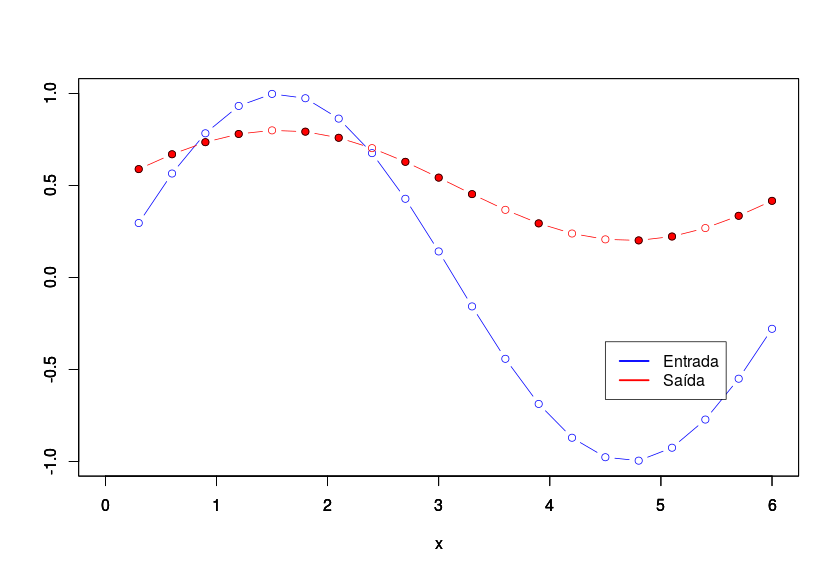
\includegraphics[width=0.7\linewidth]{Ex1a}
\caption{Amostras preenchidas foram usadas para treinamento}
\label{fig:Ex1a}
\end{figure}

\begin{figure}
	\centering
	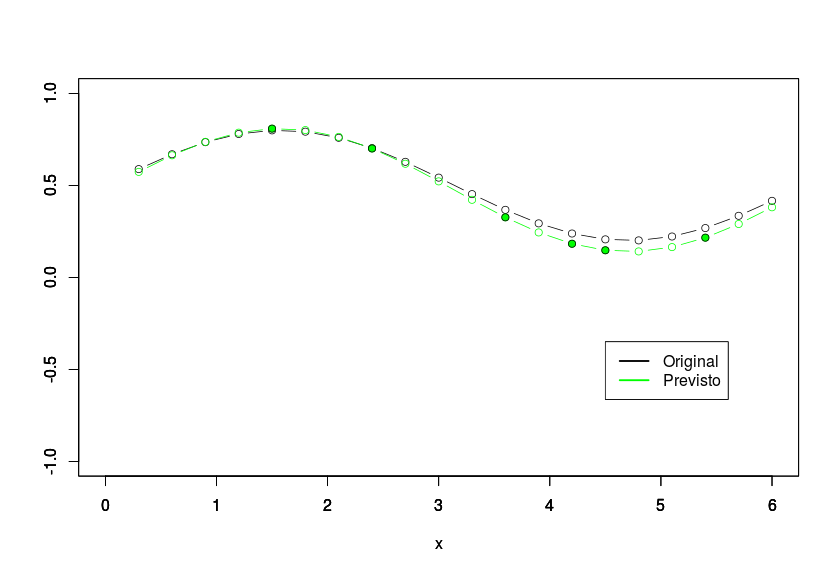
\includegraphics[width=0.7\linewidth]{Ex1b}
	\caption{Amostras preenchidas foram usadas para teste}
	\label{fig:Ex1b}
\end{figure}

\pagebreak
 
\section*{Exercício 2}
O mesmo estudante de engenharia ficou admirado com seus conhecimentos técnicos sobre \textit{Adaline} e resolveu pedir mais um favor. Ele observou que o novo sistema que ele estava trabalhando era constituído de três sinais na entrada e que a saída era uma mistura destes sinais da entrada mais um ganho. Mas este estudante não sabia muito bem como era esta mistura de sinais, a única coisa que ele sabia era que: $y = a + b*x_1 + c*x_2 + d*x3$. O aluno amostrou então os sinais na entrada e na saída para o intervalo de $[0.1\pi/:2\pi]$ e os armazenou nas variáveis $t$ (tempos amostrais), $x$ (entradas) e $y$ (saída). Sendo que a primeira coluna de $x$ é o sinal $x_1$, a segunda $x_2$ e a terceira $x_3$. Para achar os parâmetros você deverá usar $70\%$ dos dados para treinamento e $30\%$ para teste. Calcule o erro médio quadrático para as amostras de teste e plote o gráfico da saída, considerando os parâmetros encontrados, para todos os pontos da entrada. Quais são os parâmetros do modelo?
\par Obs: Use as mesmas amostras que as Figuras a seguir usaram para treinamento e teste.



\begin{figure}[h]
\centering
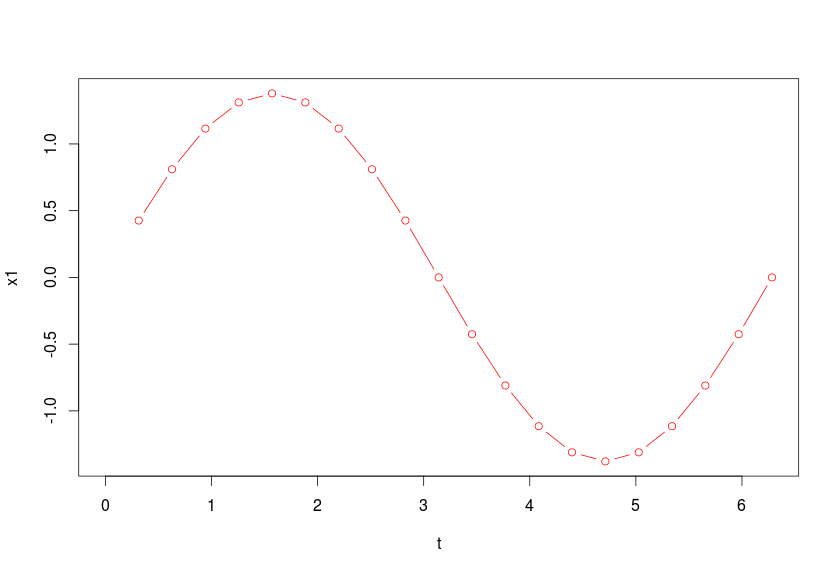
\includegraphics[width=0.32\linewidth]{x1}
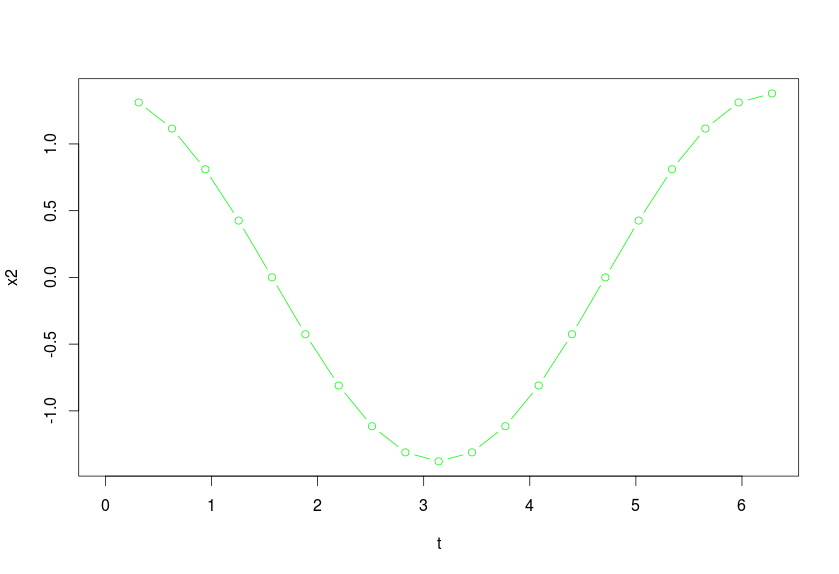
\includegraphics[width=0.32\linewidth]{x2}
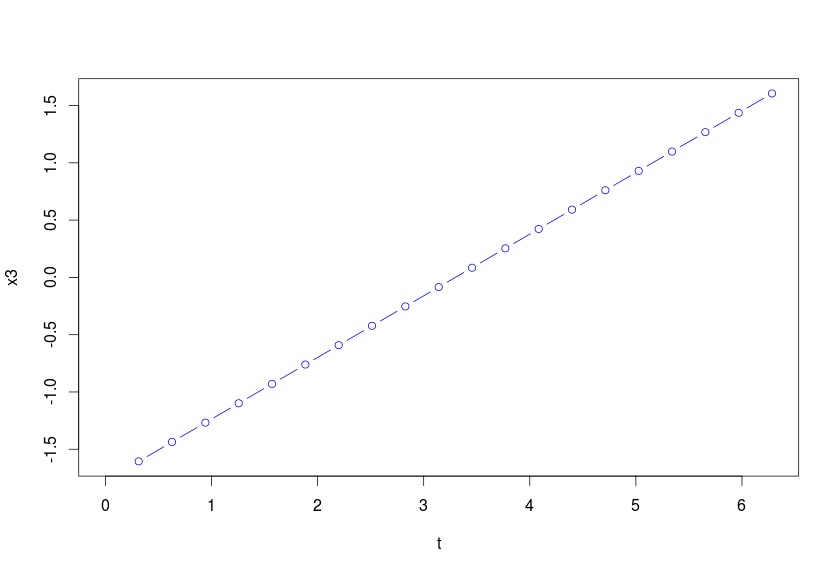
\includegraphics[width=0.32\linewidth]{x3}
\caption{Sinais de entrada $x_1$, $x_2$ e $x_3$ }
\label{fig:x1}
\end{figure}

\begin{figure}[h]
\centering
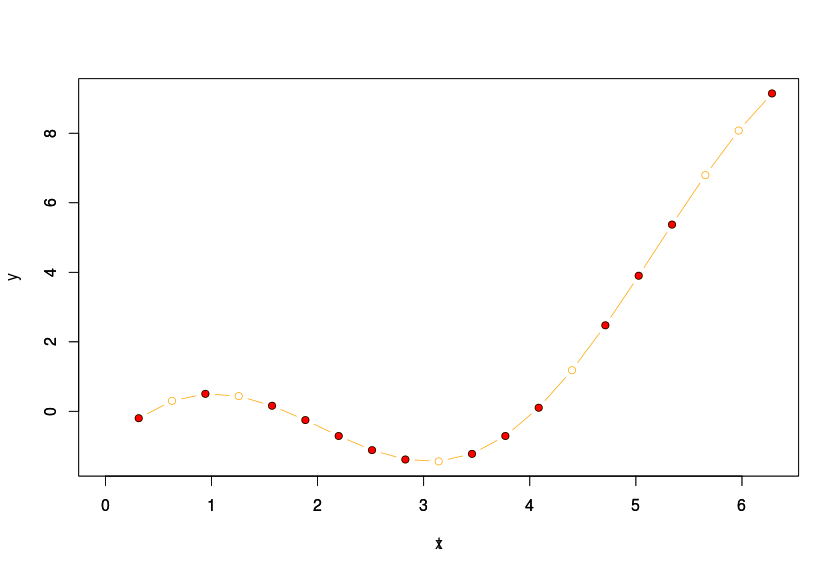
\includegraphics[width=0.6\linewidth]{y}
\caption{Saída original - amostras preenchidas foram usadas para treinamento}
\label{fig:y}
\end{figure}

\begin{figure}[h]
	\centering
	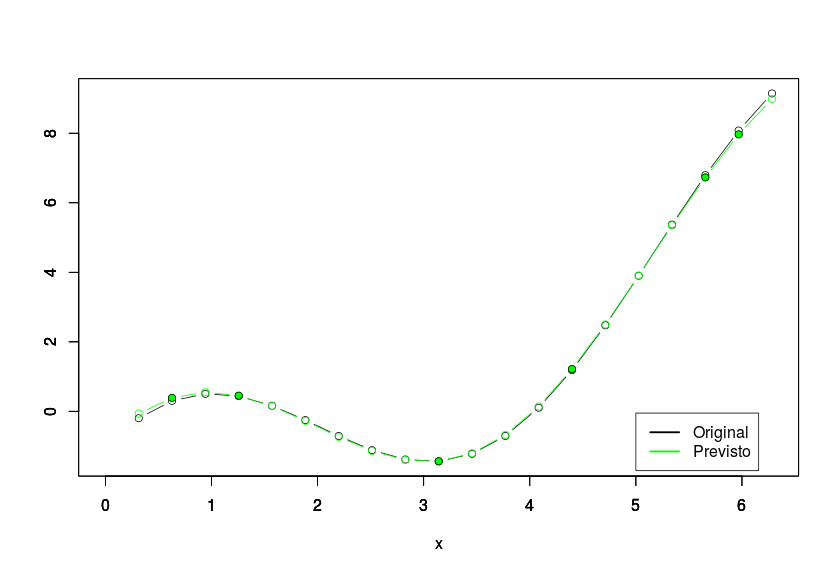
\includegraphics[width=0.6\linewidth]{yhat}
	\caption{Amostras preenchidas foram usadas para teste}
	\label{fig:yhat}
\end{figure}

\section*{Dica}
Para ler os arquivos fornecidos pelo aluno de engenharia dos exercícios use o comando.

\begin{lstlisting}
variavel<-as.matrix(read.table('nomearquivodavariavel'))
\end{lstlisting}




%----------------------------------------------------------------------------------------

\end{document}
